\documentclass[11pt]{article}\usepackage[]{graphicx}\usepackage[]{color}
%% maxwidth is the original width if it is less than linewidth
%% otherwise use linewidth (to make sure the graphics do not exceed the margin)
\makeatletter
\def\maxwidth{ %
  \ifdim\Gin@nat@width>\linewidth
    \linewidth
  \else
    \Gin@nat@width
  \fi
}
\makeatother

\usepackage{Sweavel}


\usepackage{hyperref}
\usepackage{url}
\usepackage[a4paper]{geometry}
\usepackage{a4wide}
\usepackage{float}
\usepackage[english]{babel}
\usepackage[utf8]{inputenc}
\usepackage{csquotes}
\usepackage{amsmath}
\usepackage{amssymb}
\usepackage{xspace}
\usepackage[numbers]{natbib}
\bibliographystyle{unsrtnat}
\usepackage{subcaption}
\usepackage[font={small}]{caption}
\usepackage{booktabs}
\usepackage{listings}
\usepackage{cleveref}
\usepackage{lipsum}
\newcommand{\approxtext}[1]{\ensuremath{\stackrel{\text{#1}}{=}}}
\newcommand{\matr}[1]{\mathbf{#1}}
\newcommand{\partt}[2]{\ensuremath{\dfrac{\partial {#1}}{\partial {#2}}}}
\renewcommand{\d}[1]{\ensuremath{\operatorname{d}\!{#1}}} % non-italized differentials
\newcommand{\h}[0]{\ensuremath{\hbar}} % hbar
\def\changemargin#1#2{\list{}{\rightmargin#2\leftmargin#1}\item[]}
\let\endchangemargin=\endlist 
\usepackage{amsthm}
\theoremstyle{plain}
\renewcommand{\theequation}{\thesection.\arabic{equation}}
\def\changemargin#1#2{\list{}{\rightmargin#2\leftmargin#1}\item[]}
\let\endchangemargin=\endlist    
\usepackage{xcolor}
\definecolor{Red}{rgb}{0.7,0,0}
\definecolor{Blue}{rgb}{0,0,0.8}
\usepackage{verbatim}
\def\changemargin#1#2{\list{}{\rightmargin#2\leftmargin#1}\item[]}
\let\endchangemargin=\endlist
\addtolength{\oddsidemargin}{-.35in}
\addtolength{\evensidemargin}{-.35in}
\addtolength{\textwidth}{.7in}
\usepackage{multicol}
\usepackage{afterpage}

% Stephen's stuff
\newcommand{\R}{\texttt{R}}
\newcommand{\Rfunction}[1]{{\texttt{#1}}}
\newcommand{\Robject}[1]{{\texttt{#1}}}
\newcommand{\Rpackage}[1]{{\mbox{\normalfont\textsf{#1}}}}
\usepackage{xcolor}
\definecolor{Red}{rgb}{0.7,0,0}
\definecolor{Blue}{rgb}{0,0,0.8}
\hypersetup{%
pdfusetitle,
bookmarks = {true},
bookmarksnumbered = {true},
bookmarksopen = {true},
bookmarksopenlevel = 2,
unicode = {true},
breaklinks = {false},
hyperindex = {true},
colorlinks = {true},
linktocpage = {true},
plainpages = {false},
linkcolor = {Blue},
citecolor = {Blue},
urlcolor = {Red},
pdfstartview = {Fit},
pdfpagemode = {UseOutlines},
pdfview = {XYZ null null null}
}
%% Listings
\lstset{ 
language=R,                     % the language of the code
basicstyle=\footnotesize,       % the size of the fonts that are used for the code
numbers=left,                   % where to put the line-numbers
numberstyle=\tiny\color{gray},  % the style that is used for the line-numbers
stepnumber=1,                   % the step between two line-numbers. If it's 1, each line will be numbered
numbersep=5pt,                  % how far the line-numbers are from the code
backgroundcolor=\color{white},  % choose the background color. You must add \usepackage{color}
showspaces=false,               % show spaces adding particular underscores
showstringspaces=false,         % underline spaces within strings
showtabs=false,                 % show tabs within strings adding particular underscores
rulecolor=\color{black},        % if not set, the frame-color may be changed on line-breaks within not-black text (e.g. commens (green here))
tabsize=2,                      % sets default tabsize to 2 spaces
captionpos=b,                   % sets the caption-position to bottom
breaklines=true,                % sets automatic line breaking
breakatwhitespace=false,        % sets if automatic breaks should only happen at whitespace
title=\lstname,                 % show the filename of files included with \lstinputlisting;
% also try caption instead of title
keywordstyle=\color{Blue},      % keyword style
commentstyle=\color{orange},    % comment style
stringstyle=\color{Red},        % string literal style
escapeinside={\%*}{*)},         % if you want to add a comment within your code
morekeywords={*,...}            % if you want to add more keywords to the set
} 
\usepackage{graphicx}



%%% Document specific
\newcommand{\course}{Structural Biology}
\newcommand{\ass}{3}
\newcommand{\term}{Lent term 2017}
%\bibliography{pga1}

%%% Title page
\title{
  \bf \course: Assignment \ass \\[1em]
  \small{University of Cambridge}
}

\author{Henrik Åhl}
\date{\today}
\renewcommand{\textfraction}{0.05}
\renewcommand{\topfraction}{0.8}
\renewcommand{\bottomfraction}{0.8}
\renewcommand{\floatpagefraction}{0.75}

%%% Actual document
\begin{document}
\date{\today}
\maketitle
\setcounter{page}{1}


% \date{\today}
\maketitle
% \begin{abstract}
% {\bf 
%   %\begin{changemargin}{-.8cm}{-.8cm}
%   This is an abstract abstract.
% }
% \end{abstract}

\begin{multicols*}{2}
\section*{Preface}
This is an assignment report in connection to the \textit{\course}
module in the Computational Biology course at the University of Cambridge,
\term. All related code is as of \date{\today} available through a
Github repository by contacting \href{mailto:hpa22@cam.ac.uk}{hpa22@cam.ac.uk}.

\section*{Exercises}
  \begin{figure*}[p]
    \centering
    \phantom{p}
    \vspace{-6cm}
    \begin{subfigure}[b]{.49\textwidth}
      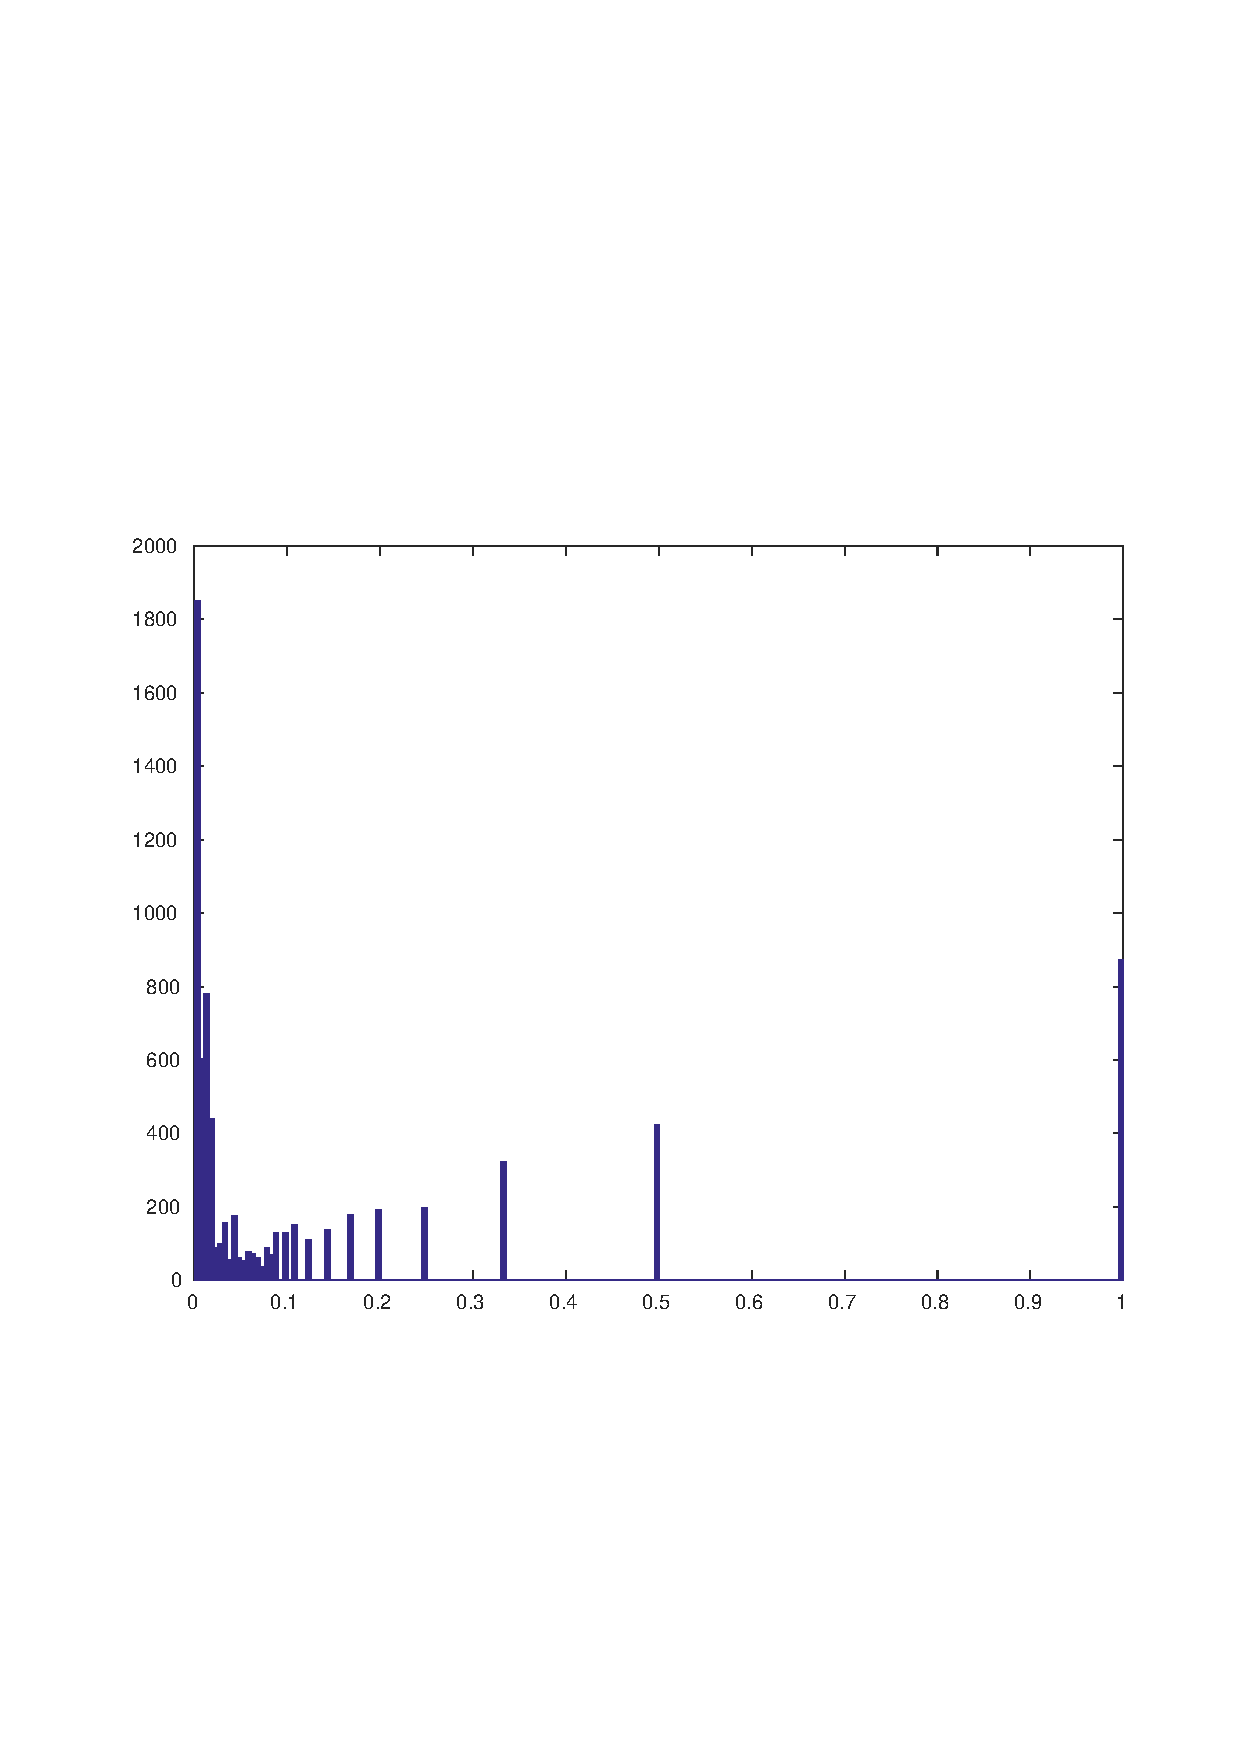
\includegraphics[width=\textwidth, trim= 4cm 9.5cm 4cm 4cm, clip]{../figures/this_thing_histogram}
      \caption{ }
      \label{fig:human_fig1}
    \end{subfigure}~
    \begin{subfigure}[b]{.5\textwidth}
      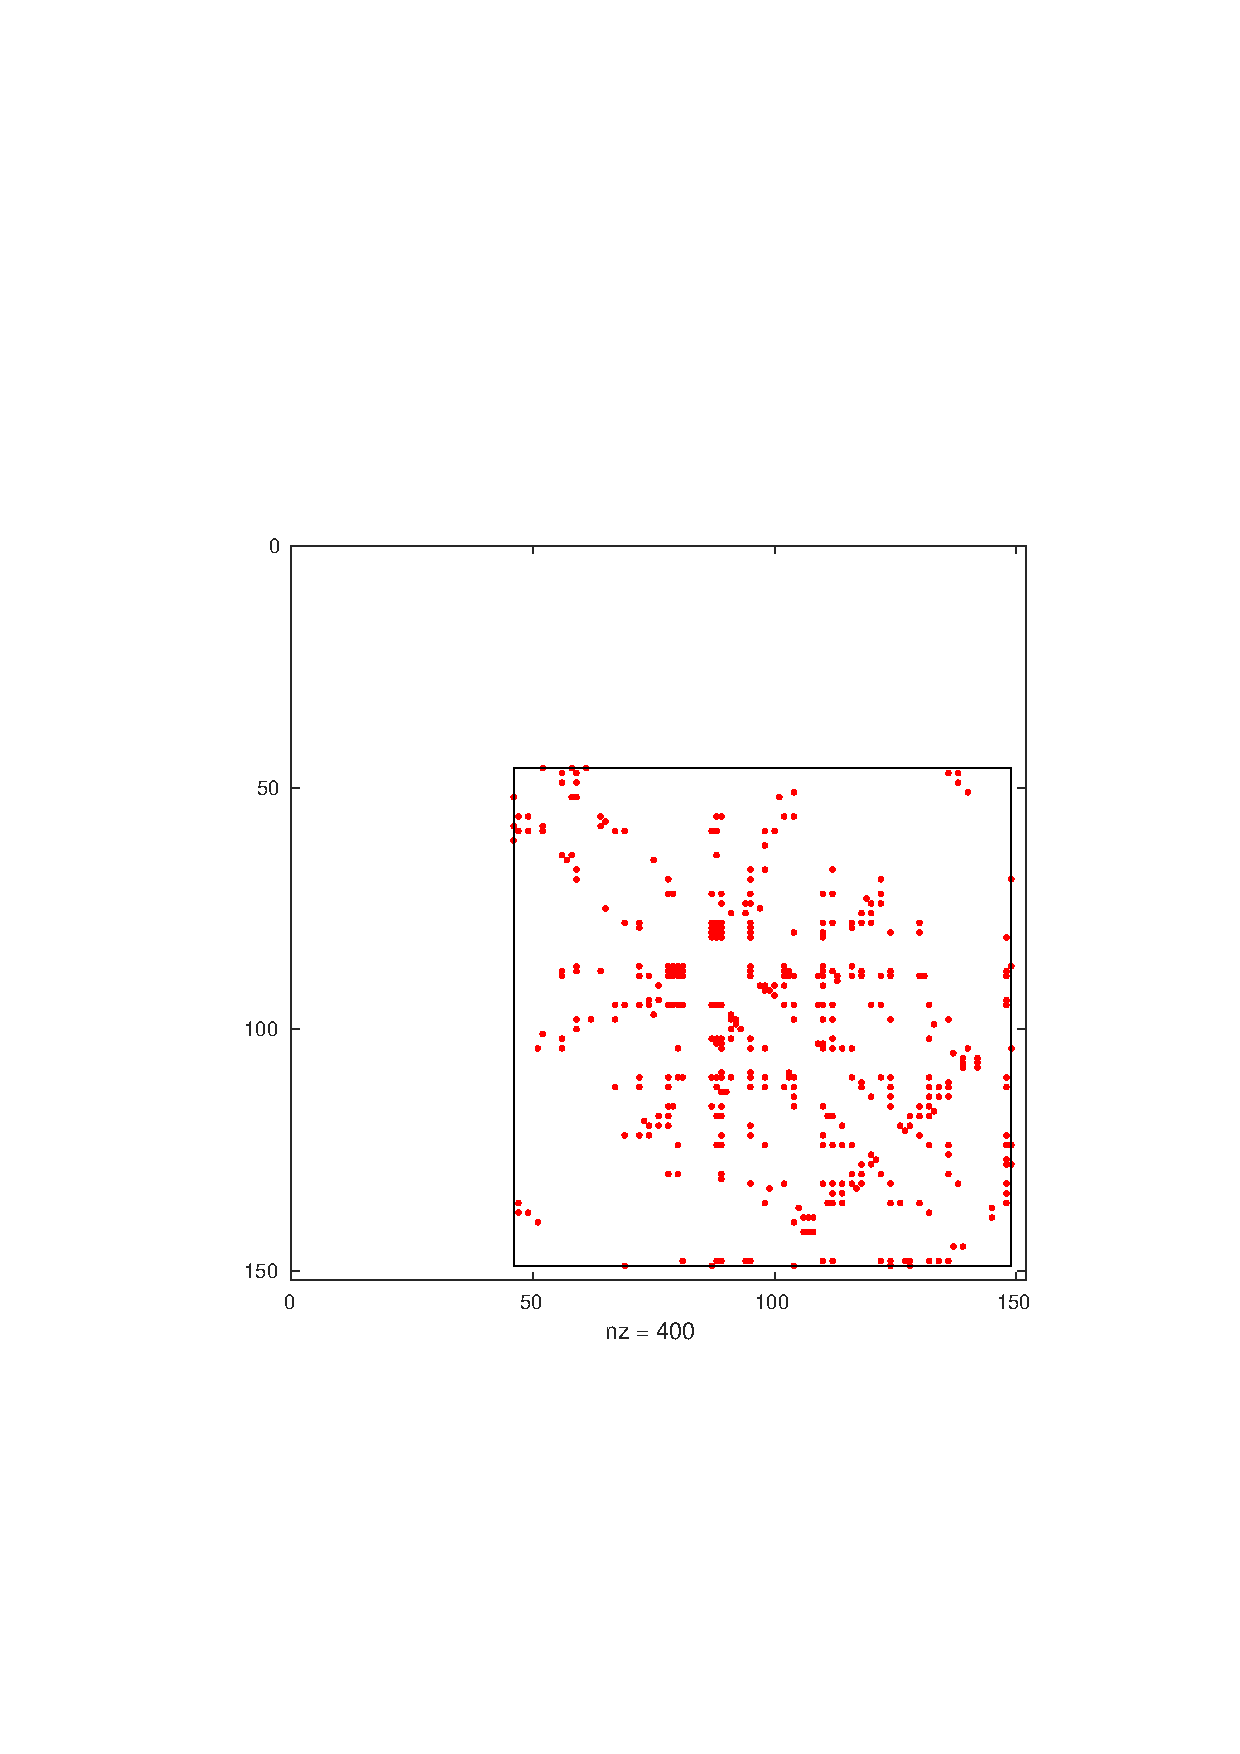
\includegraphics[width=\textwidth, trim=2cm 7cm 2cm 7cm, clip]{../figures/CADH1_HUMAN_e3_n2_m40_Predicted_Constraints}
      % 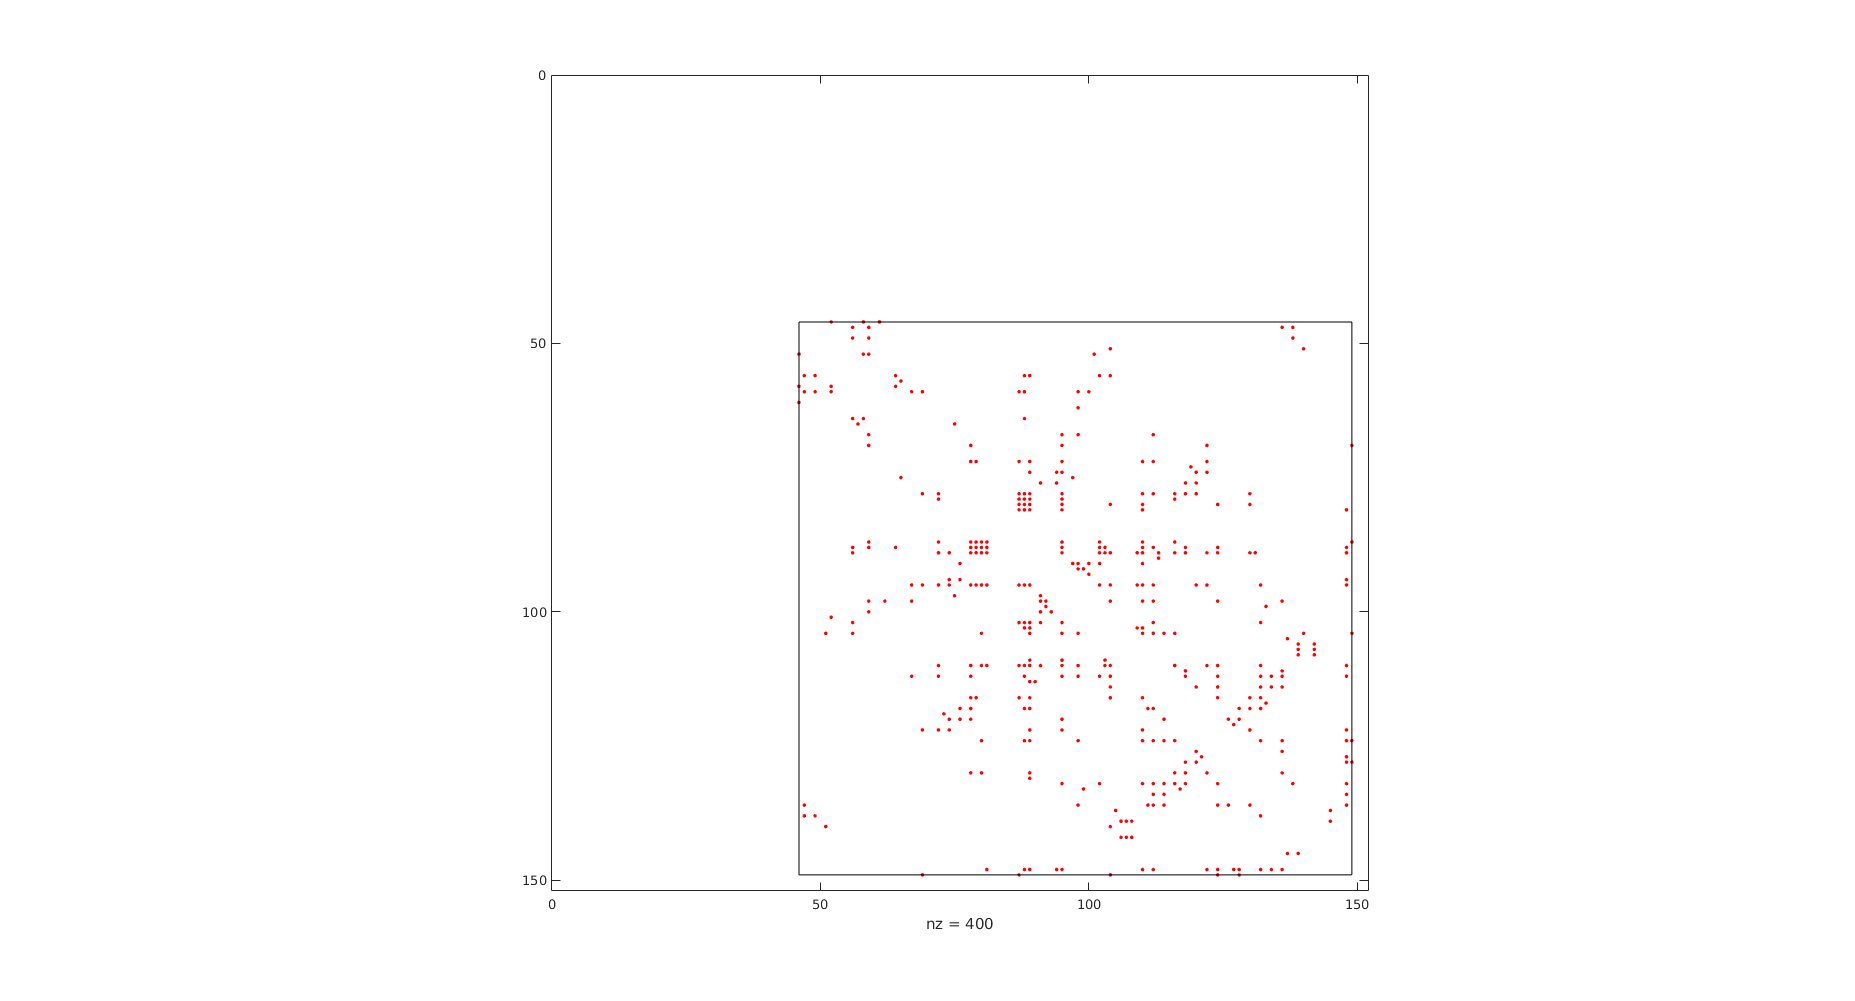
\includegraphics[width=\textwidth, trim= 10cm 0 10cm 0, clip]{../figures/fig2}
      \caption{ }
      \label{fig:human_fig2}
    \end{subfigure}\\
    \begin{subfigure}[b]{.49\textwidth}
      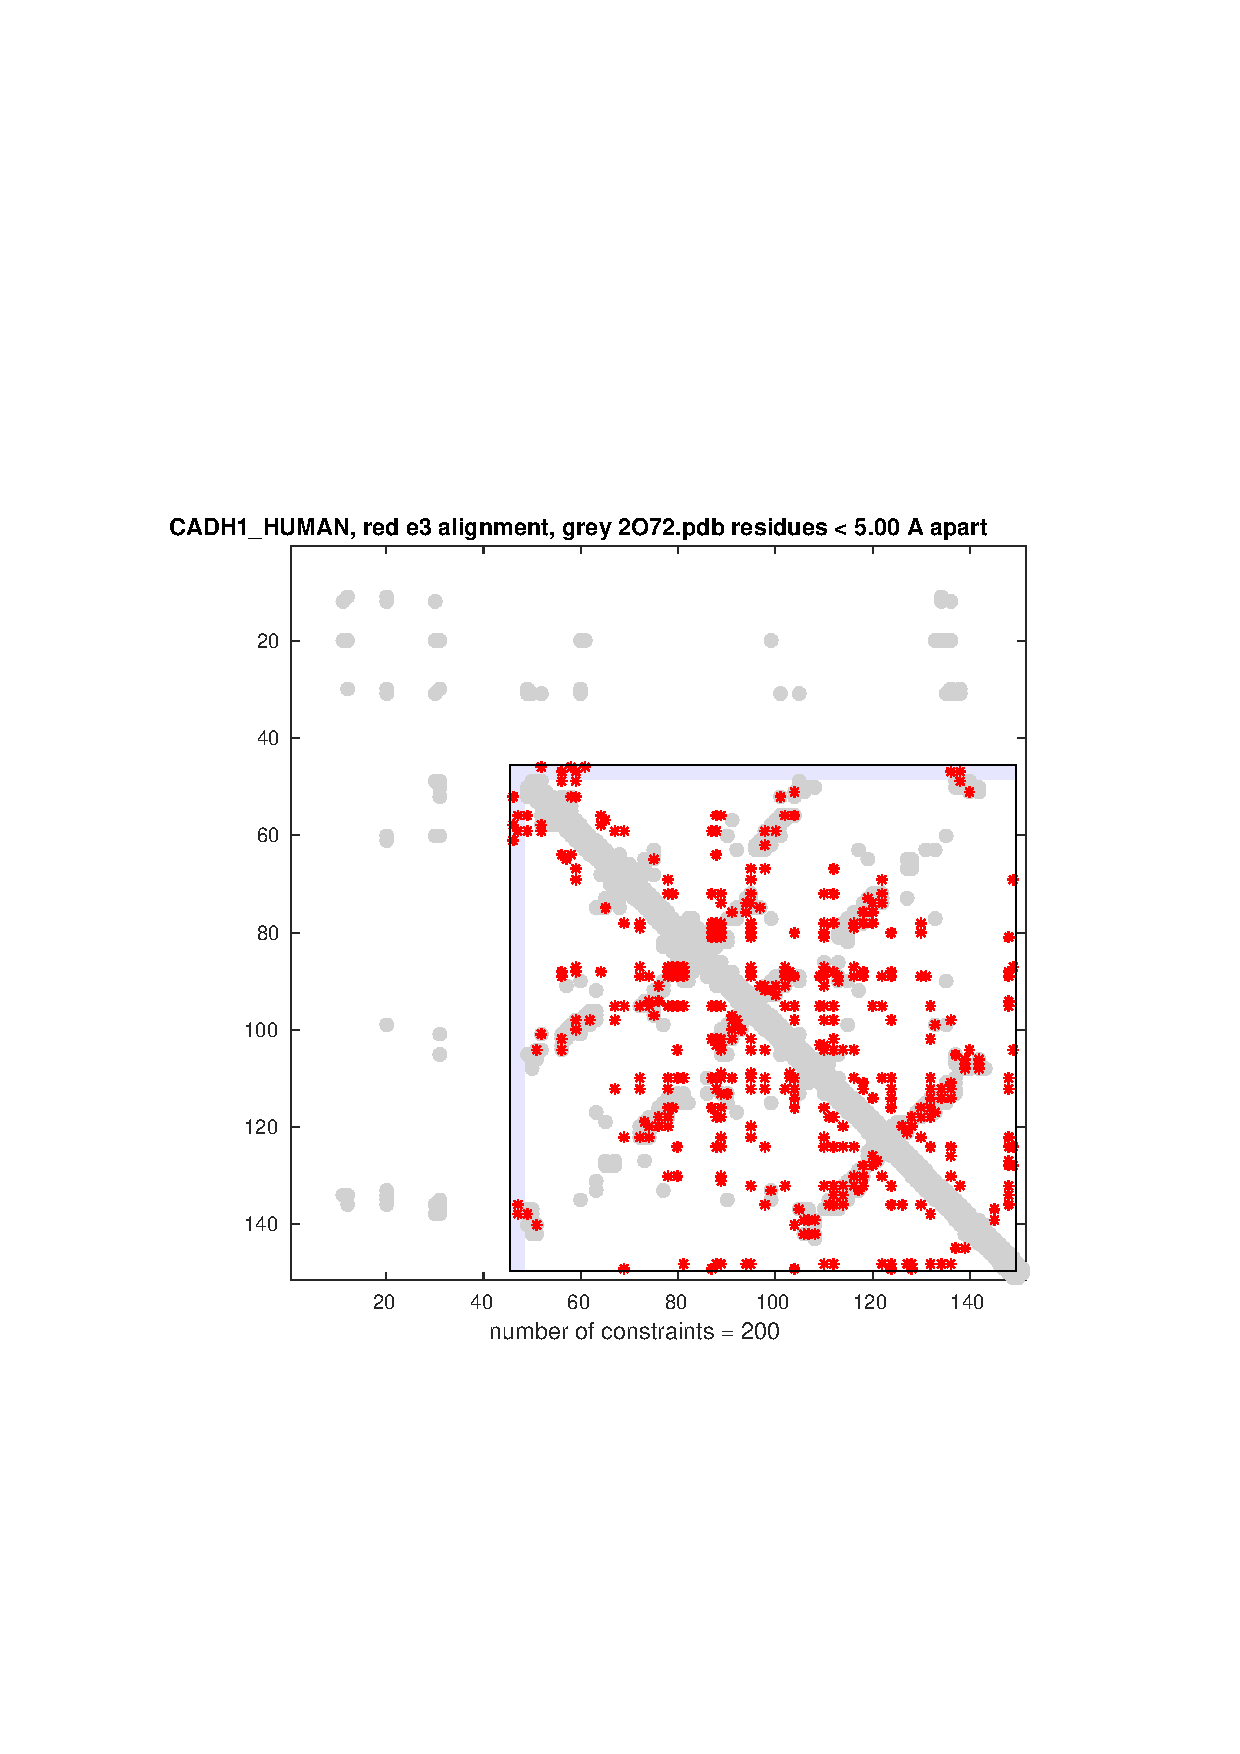
\includegraphics[width=\textwidth, trim= 2cm 7cm 2cm 0cm, clip]{../figures/CADH1_HUMAN_e3_n2_m40_FPplot}
      \caption{ }
      \label{fig:human_fig3}
    \end{subfigure}~
      \begin{subfigure}[b]{.5\textwidth}
      % 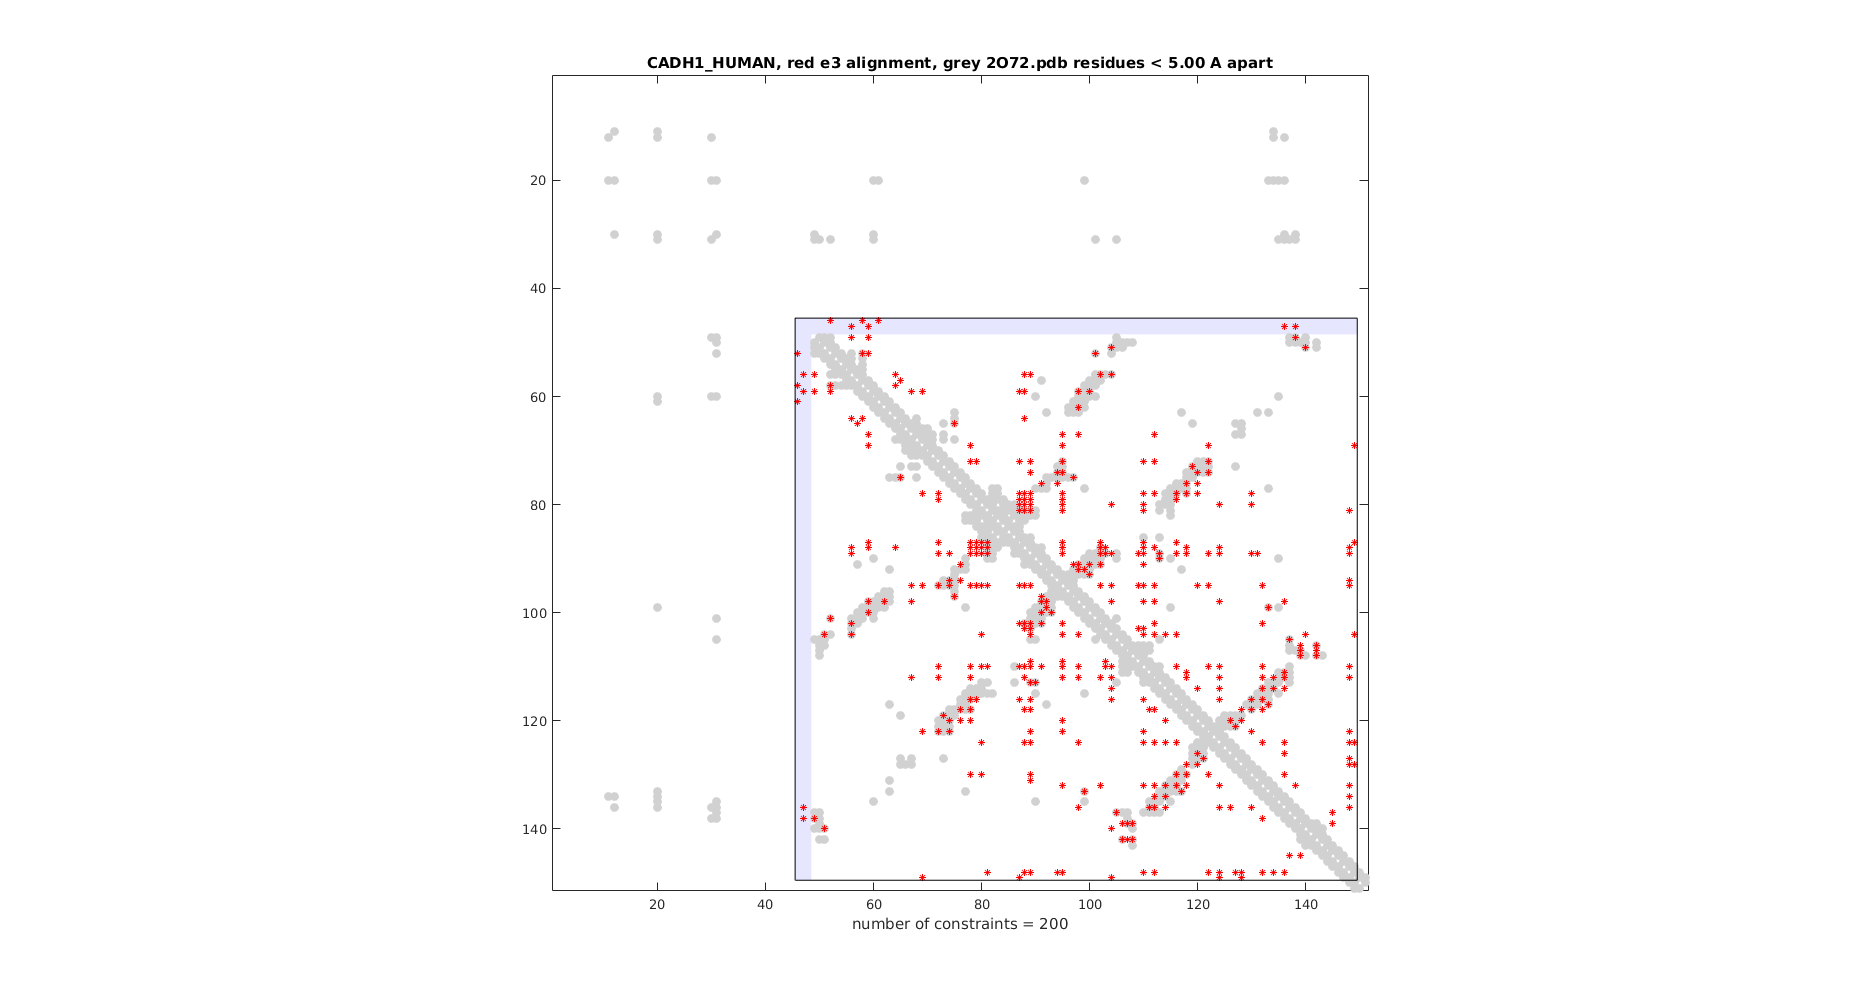
\includegraphics[width=\textwidth, trim= 10cm 0cm 10cm 0, clip]{../figures/fig4 }
      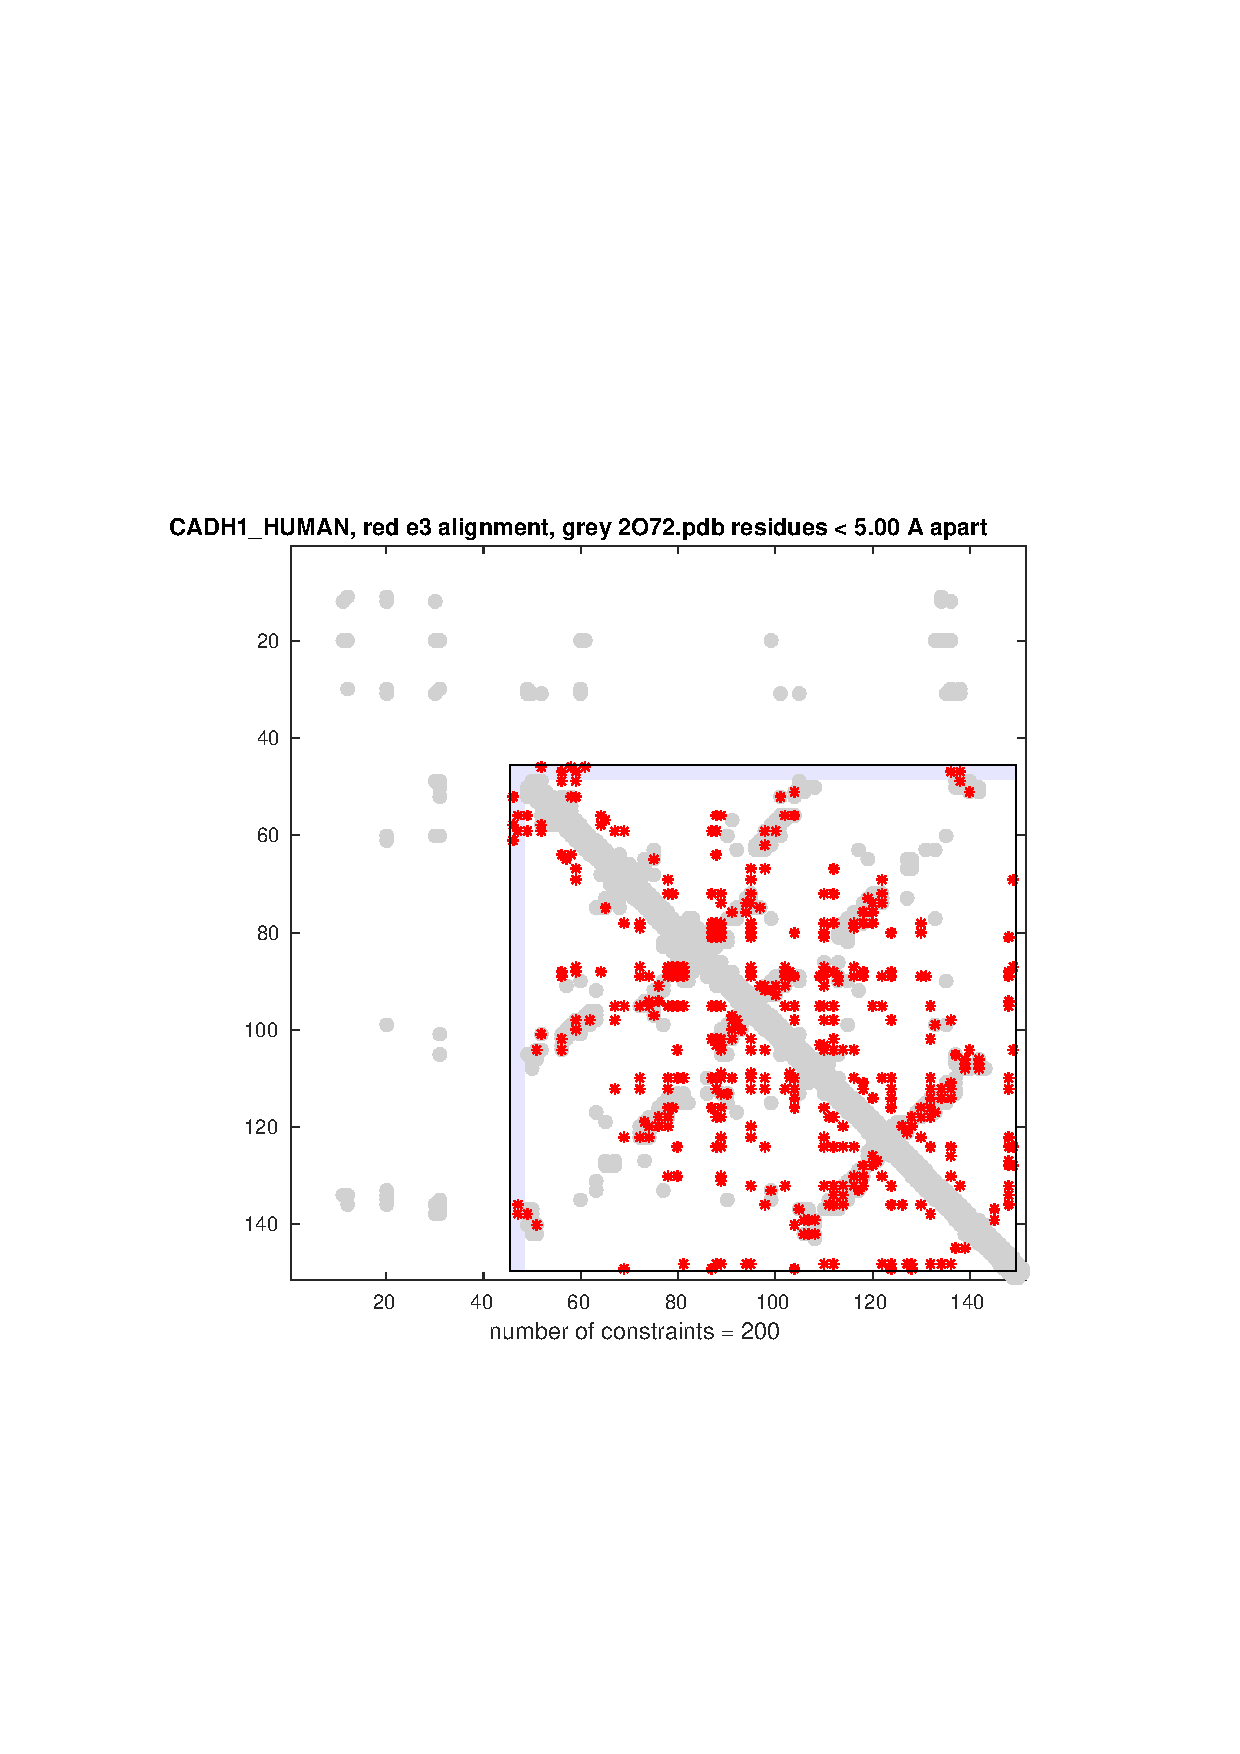
\includegraphics[width=\textwidth, trim=2cm 7cm 2cm 7cm, clip]{../figures/CADH1_HUMAN_e3_n2_m40_Cmap_200}
      \caption{ }
      \label{fig:human_fig4}
    \end{subfigure}%
    \caption{Figure of figures}
    \label{fig:init_figures}
  \end{figure*}


  \begin{figure*}[p]
    \centering
    \phantom{p}
    \vspace{-6cm}
    \begin{subfigure}[b]{.49\textwidth}
      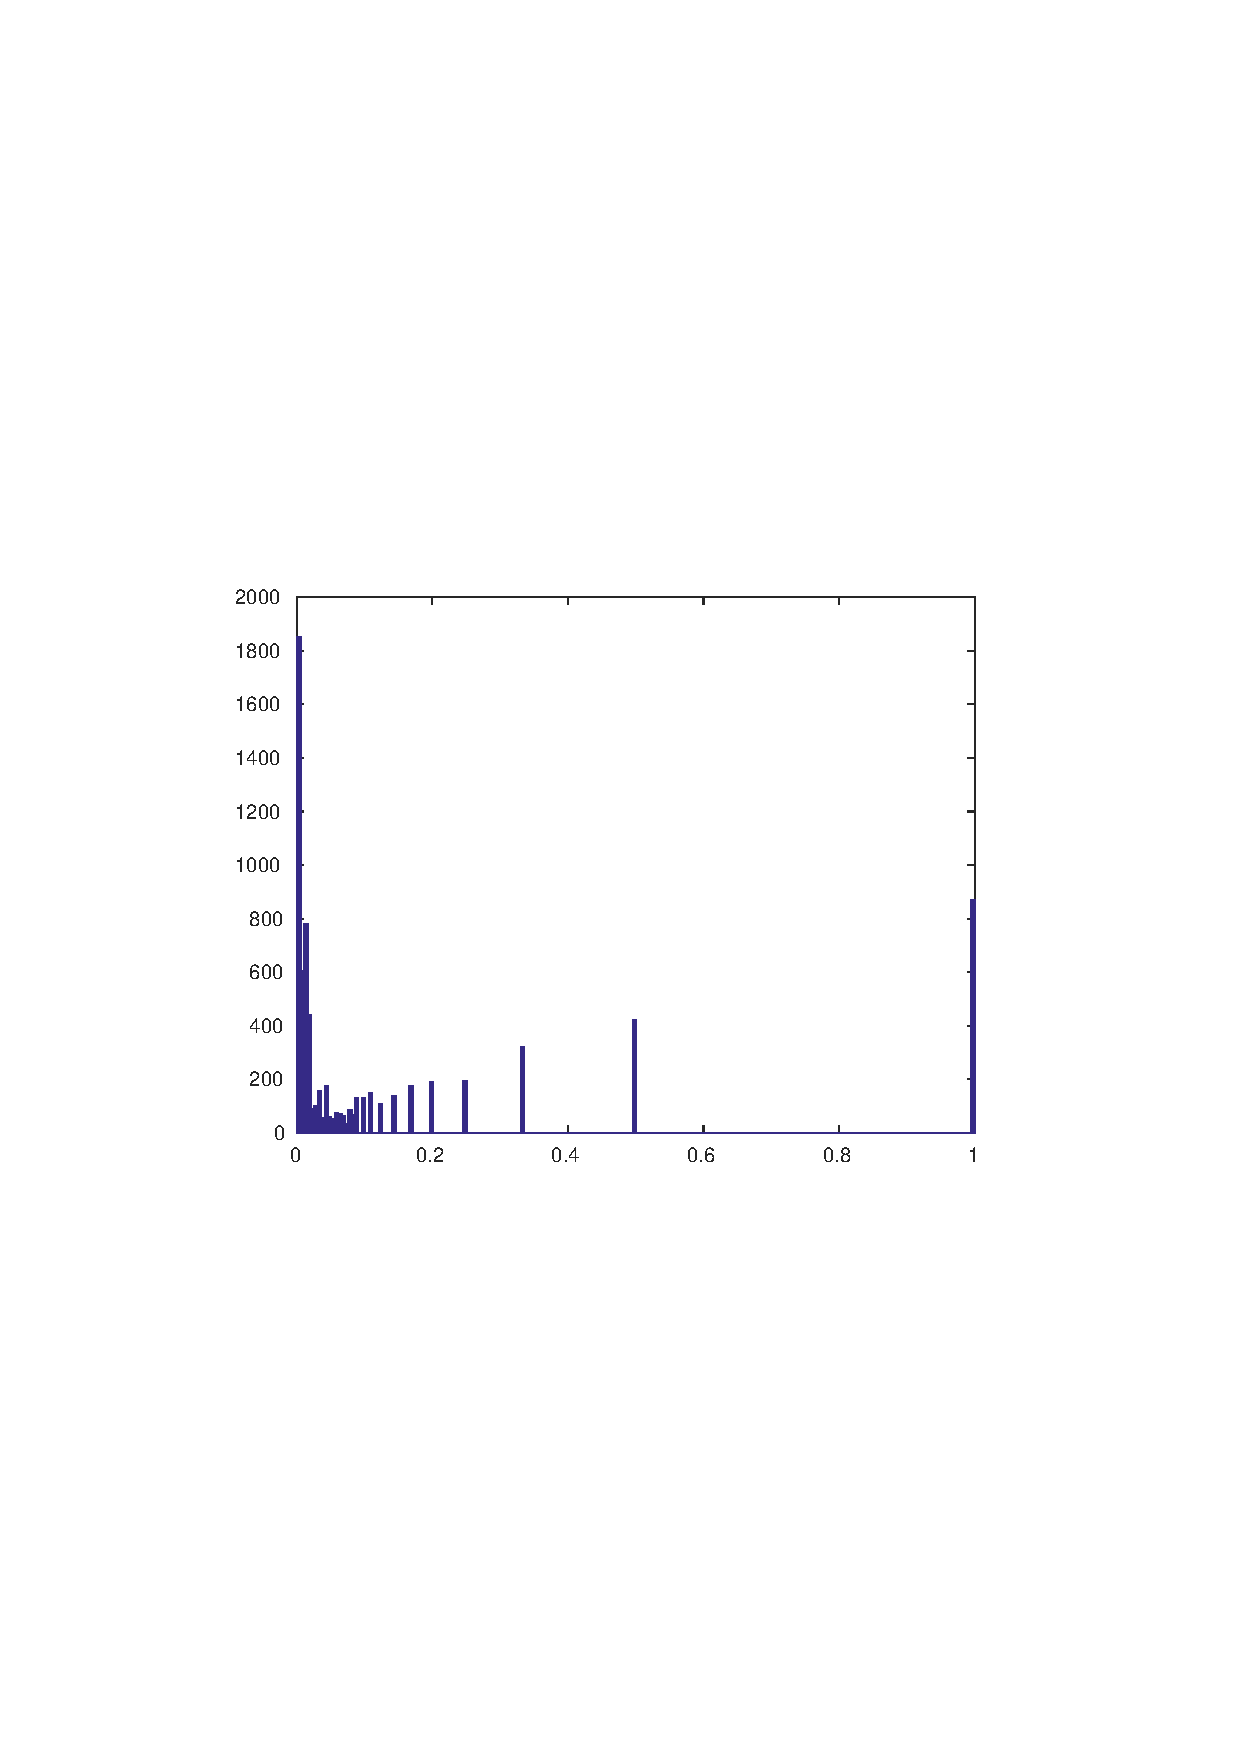
\includegraphics[width=\textwidth, trim= 4cm 9.5cm 4cm 4cm, clip]{../figures/DYR_ECOLI_e3_n2_m40_histogram}
      \caption{ }
      \label{fig:fig1}
    \end{subfigure}~
    \begin{subfigure}[b]{.5\textwidth}
      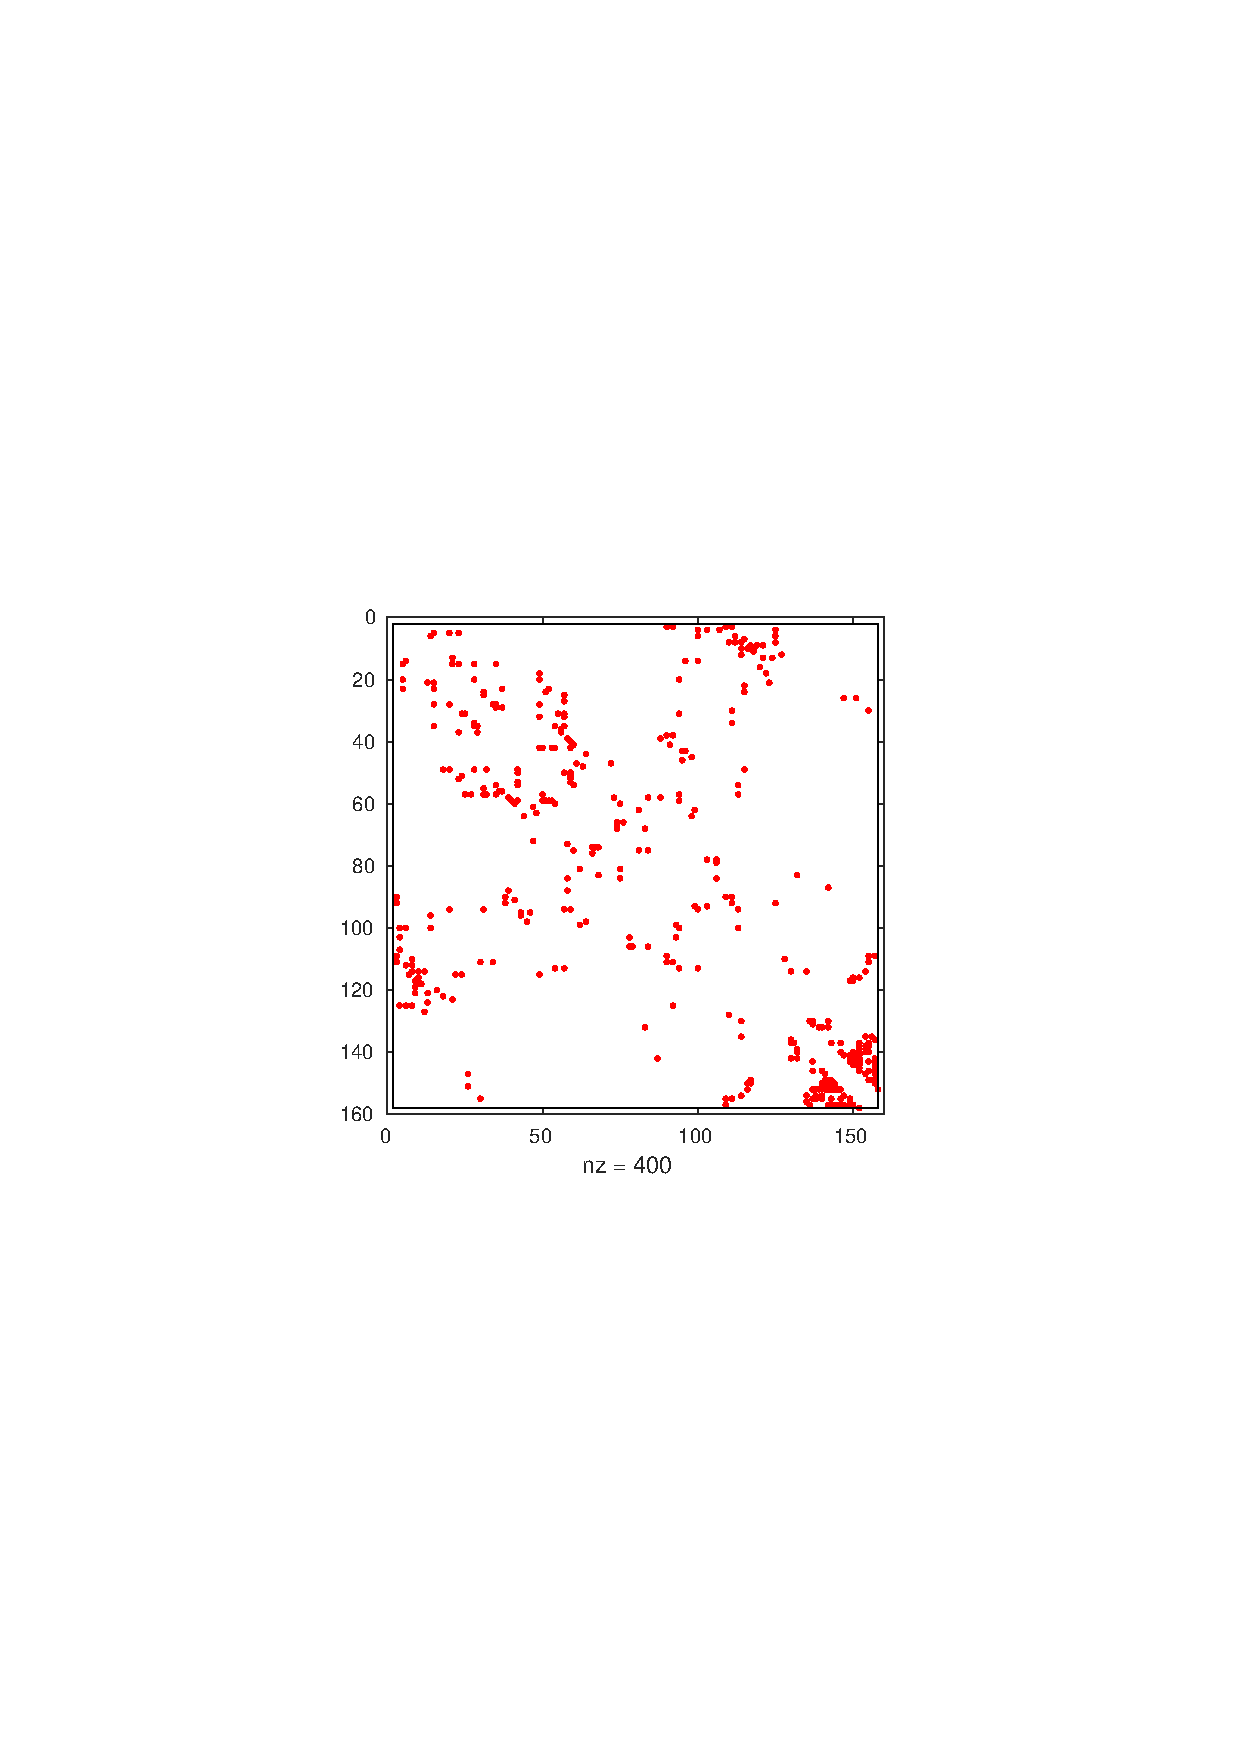
\includegraphics[width=\textwidth, trim=2cm 7cm 2cm 7cm, clip]{../figures/DYR_ECOLI_e3_n2_m40_Predicted_Constraints}
      % 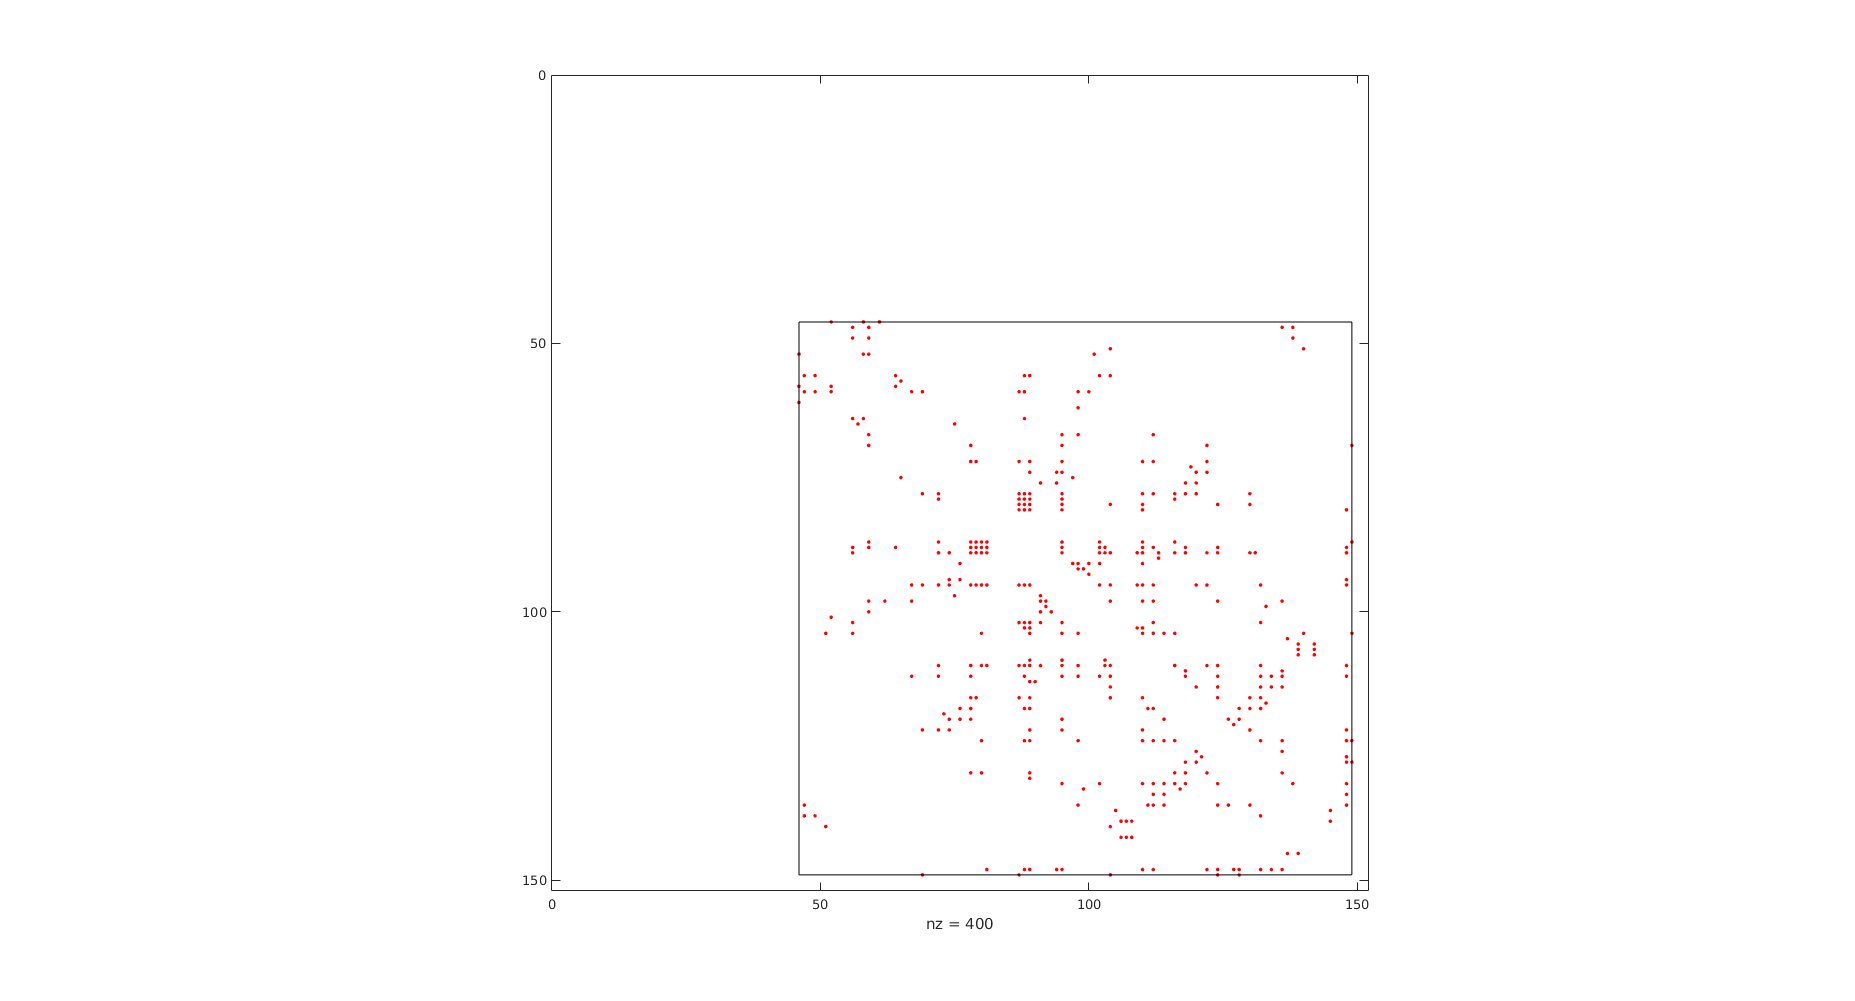
\includegraphics[width=\textwidth, trim= 10cm 0 10cm 0, clip]{../figures/fig2}
      \caption{ }
      \label{fig:fig2}
    \end{subfigure}\\
    \begin{subfigure}[b]{.49\textwidth}
      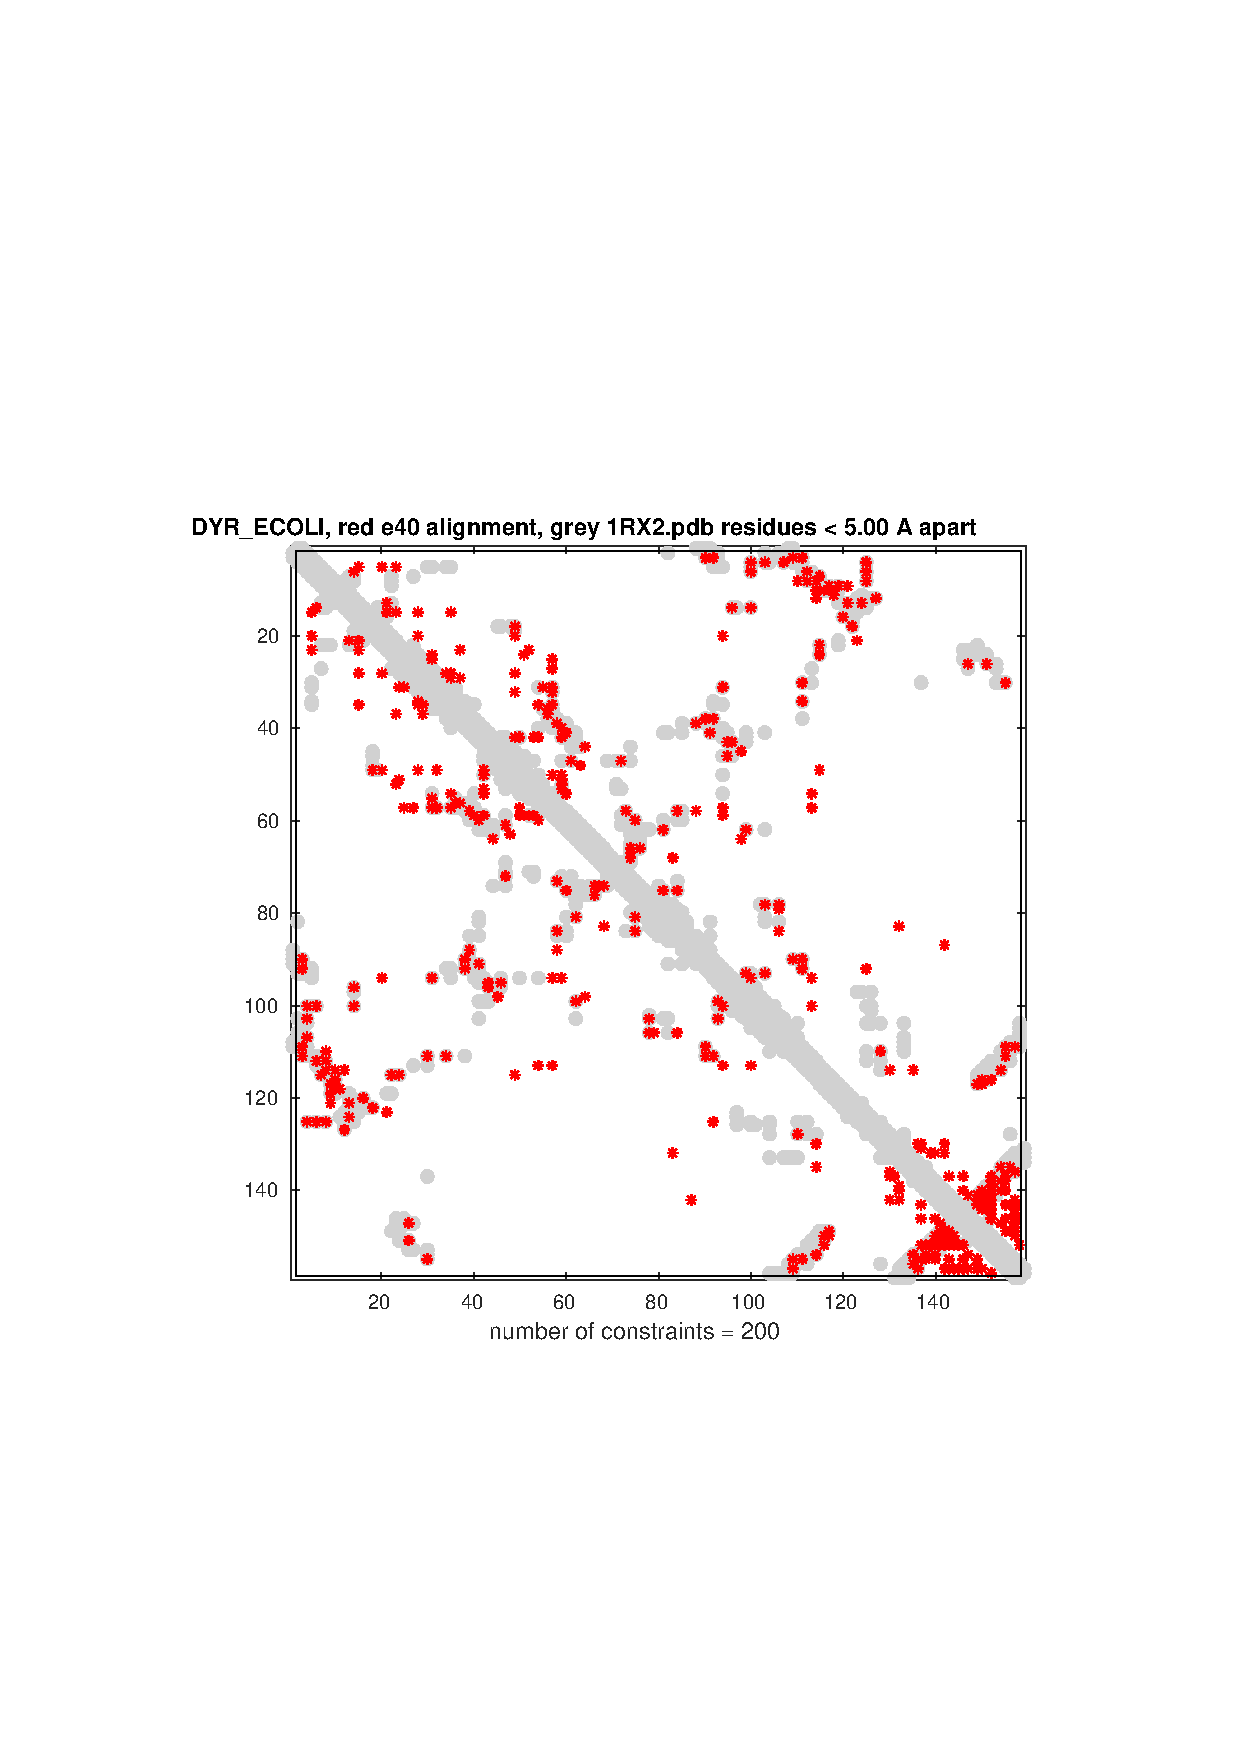
\includegraphics[width=\textwidth, trim= 2cm 7cm 2cm 0cm, clip]{../figures/DYR_ECOLI_e3_n2_m40_FPplot}
      \caption{ }
      \label{fig:fig3}
    \end{subfigure}~
      \begin{subfigure}[b]{.5\textwidth}
      % 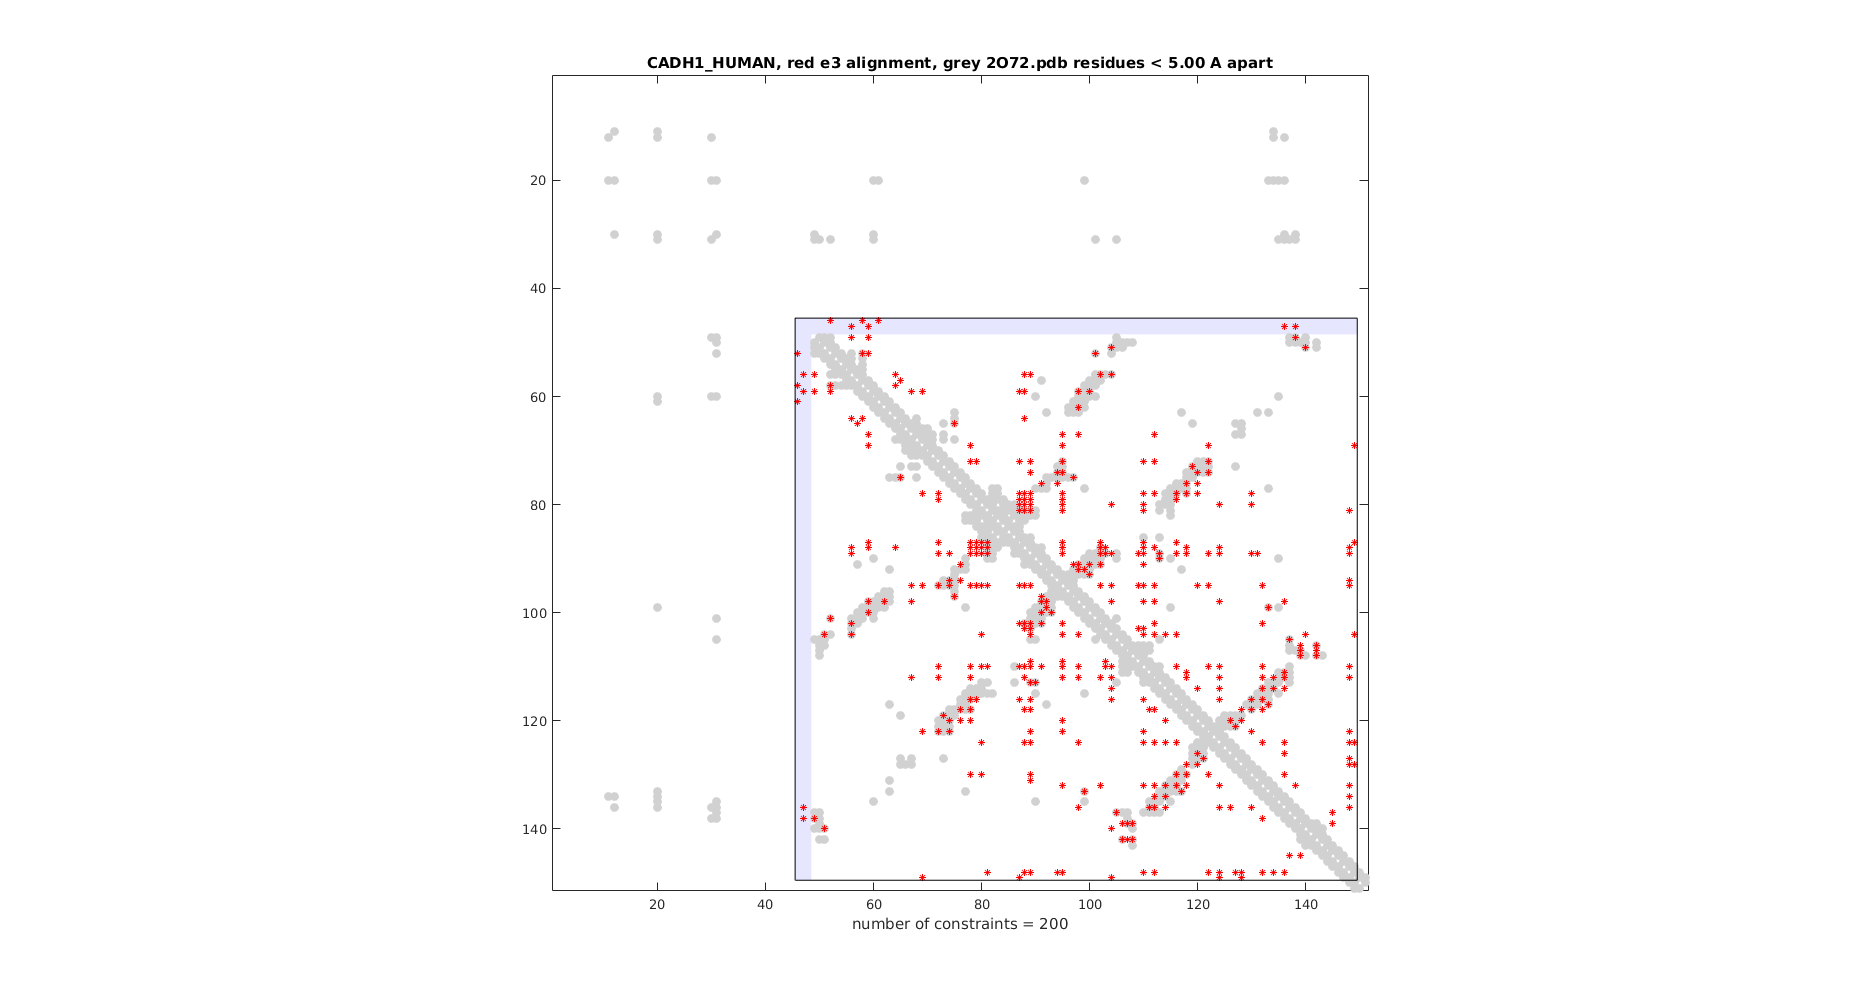
\includegraphics[width=\textwidth, trim= 10cm 0cm 10cm 0, clip]{../figures/fig4 }
      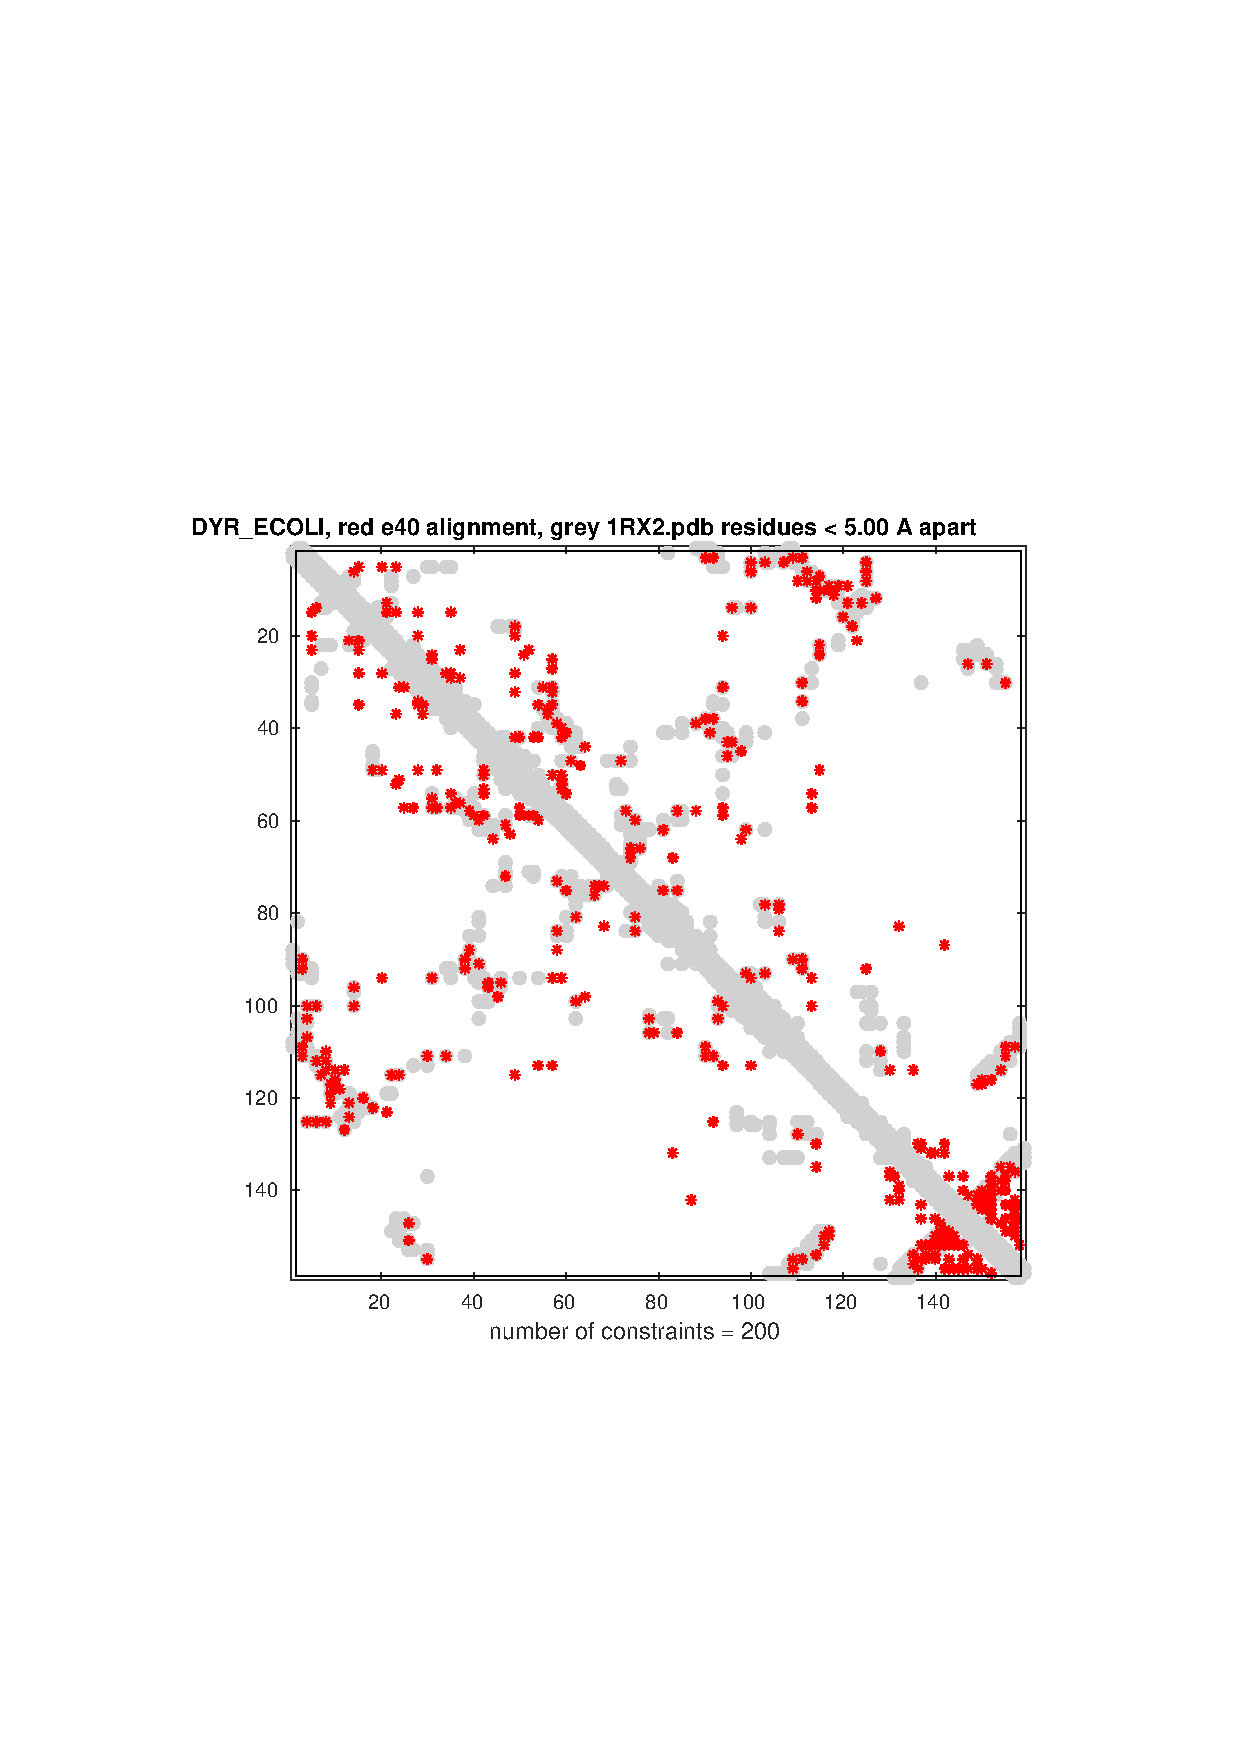
\includegraphics[width=\textwidth, trim=2cm 7cm 2cm 7cm, clip]{../figures/DYR_ECOLI_e3_n2_m40_Cmap_200}
      \caption{ }
      \label{fig:fig4}
    \end{subfigure}%
    \caption{Figure of figures}
    \label{fig:init_figures}
  \end{figure*}

% this code reads in the output of get_constraints.m and compares it to the
% experimentally solved crystal structure of a protein sequence from the
% alignment. 

% Fig 3: plots min all atom distance against DI ranking (x axis).
% Fig 2: plots the distance in structure for each pair vs the rank of the pair
% Fig 3/4:  contact map overlay plotsmia
% 3: 	plot(plotRows,plotCols,'o','MarkerSize',6,'MarkerFaceColor',CRYSTAL_CONTACT_COLOR,'MarkerEdgeColor',CRYSTAL_CONTACT_COLOR);
% 4: 	plot(plotRows,plotCols,'*','MarkerSize',4,'MarkerFaceColor',EIC_COLOR,'MarkerEdgeColor',EIC_COLOR);

% Figure 1 shows the distribution of normalised frequency of the different amino acids in each respective column.
%1
\paragraph{1}
\Cref{fig:fig1} shows the frequency distribution of the weighted pairwise matches between sequences, given that their similarity fraction is $> 70 \%$. For every sequence, the number of \textit{other} sequences with a $> 70~\%$ similarity to this adds an increment of one to the parameter $d_i$ in the equation 
\begin{equation*}
  W_i = \dfrac{1}{1 + d_i}.
\end{equation*}
 That is, we downscale for weights for the sequences that are high in abundance (given our similarity threshold), since they add little additional information to what is already known. This means that the histogram we see in \cref{fig:fig1} is given in fractions of $1, 1/2, 1/3, \ldots$, as this shows the frequency distribution of these weights.

\Cref{fig:fig2} shows the predicted protein contact map between the residues in each sequence, i.e.\ how correlated certain positions are with each other based on the evolutionarily inferred contact (EIC) scores. \Cref{fig:fig3} in turn depicts the minimal distance between the amino acids in the crystal as a function of the corresponding DI rank. Lastly, \cref{fig:fig4} shows the overlap between the experimentally observed structure and the predicted tertiary  interactions.  

%2
\paragraph{2}
The accuracy of the method is directly dependent on the quality of the sequence alignment. As these often utilize multiple heuristic simplification in order to improve speed, longer sequences are bound to align improperly. While functionally important segments should be better conserved and align better, there is always the risk of error in this, which makes the method as a whole reliant both on the alignment method used, and the numbers of sequences aligned. Using more elaborate approaches such as direct dynamic programming is instead feasible when analysing smaller and/or fewer proteins. While cumbersome and time-consuming, one can also, by using prior information of how the sequences in question differ, tailor the alignment according to data at hand in order to improve upon this. Another obvious problem is the quality of the experimental correlations, which depends inherently on the sample size and resolution of the protein in question. This might obfuscate lowly correlated but functionally important residues, which affect the overall structure and stability by long-range interactions or simply aid the protein in folding into the native state. Lastly, sequence alignment data does not take into account environmental factors, such as how certain parts of the protein might interact with other molecules in a way such that protein functionality invisible in the primary sequence is conserved or maintained. If this is the case, and this functionality is not conserved spatially in relation to other residues, this might as well be obfuscated. In other words, as a high score indicates contact, a low score must not necessarily mean no contact between residues.

% REWRITE ^

% 3
\paragraph{3}
% Write this

% 4
\paragraph{4}
The parameter $\theta$ sets, as previously hinted, the similarity percentage cutoff between sequences. In our case, as it is set to $\theta = 0.3$, only sequences with more than $1.0 - 0.3 = 0.7 = 70~\%$ similarity will be processed when calculating the weights. This makes it so that, according to the aforementioned equation, sequences which are very similar will add less to the corresponding weights, as the information is duplicated in several parts of the input data, which here are the homologues. By doing so, we smoothen our distribution of weights, and thus makes it more variable due to smaller variation.

% question 5
\paragraph{5}
Pseudocounts are used for smoothing distributions in particular when some specific probabilistic outcomes are unlikely to occur in relation to the size of the data set. In the case of amino acids, this could be to add and increment to the number of times a residue has been observed. For each amino acid, a different increment would be attributed, based on a prior estimates of how likely they are to appear. This approach is done in order to avoid sharp peaks in the distribution of values in for example a position weight matrix, where small changes in the number of observations would have large effects the resulting value, in the case where pseudocounts are not used. In practice, pseudocounts can be set to calculate the posterior estimator of the mean as
$$
\theta^{PME}_i = \dfrac{n_i + \alpha_i}{|\mathbf n| + |\mathbf \alpha |}
$$
where $n_i$ is the number of observations of component $i$, and $\alpha$ is the pseudocounts for that component~\cite{durbin1998biological}.

% The pseudocounts roughly reflect the chances of seeing the amino acid in a context in which we have not previously seen it. A low pseudocount for an amino acid means that the amino acid is not often seen in a context in which some other amino acid has already been observed. If the pseudocount is lower than we would expect from the background probabilities, then the amino acid must be more highly conserved than other amino acids. Using this reasoning, we expect that G, P, W, and C are often highly conserved. Using symmetric reasoning for pseudocounts that are higher than expected from the background probabilities,   we also expect that M, Q, and S are less conserved than other amino acids.


\bibliography{references}
\end{multicols*}
\end{document}
